\section{section}\label{section}

こちらはアブスト \emph{斜体} \textbf{太字} \textbf{\emph{太字斜体}}

\subsection{subsection}\label{subsection}

\begin{itemize}
\tightlist
\item
  箇条書き
\item
  箇条書き
\end{itemize}

\subsubsection{subsubsection}\label{subsubsection}

\begin{enumerate}
\def\labelenumi{\arabic{enumi}.}
\tightlist
\item
  数字の箇条書き
\item
  数字の箇条書き
\end{enumerate}

\section{図の貼り方}\label{ux56f3ux306eux8cbcux308aux65b9}

図\ref{fig:sample}にサンプル図を示す.

\begin{figure}[ht]
\centering
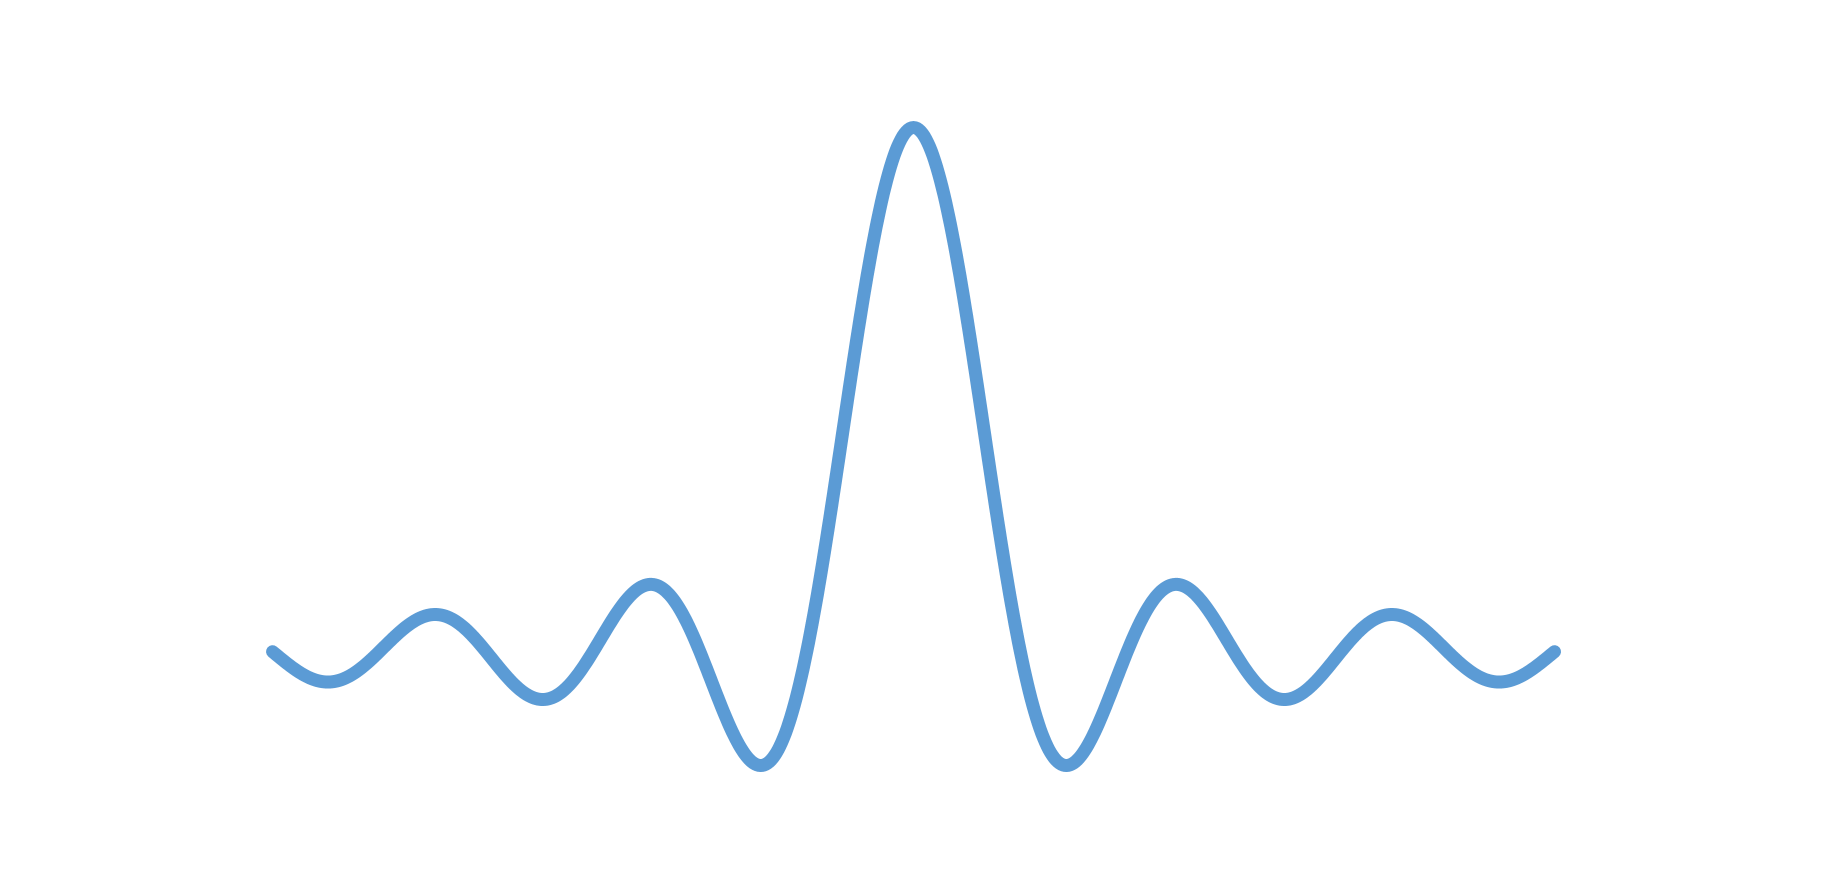
\includegraphics[width=8.00000cm]{./fig/sample.png}
\caption{Sample\label{fig:sample}}
\end{figure}

\subsection{図を横に並べる}\label{ux56f3ux3092ux6a2aux306bux4e26ux3079ux308b}


\begin{figure}[ht]
\centering
\begin{tabular}[]{@{}cc@{}}

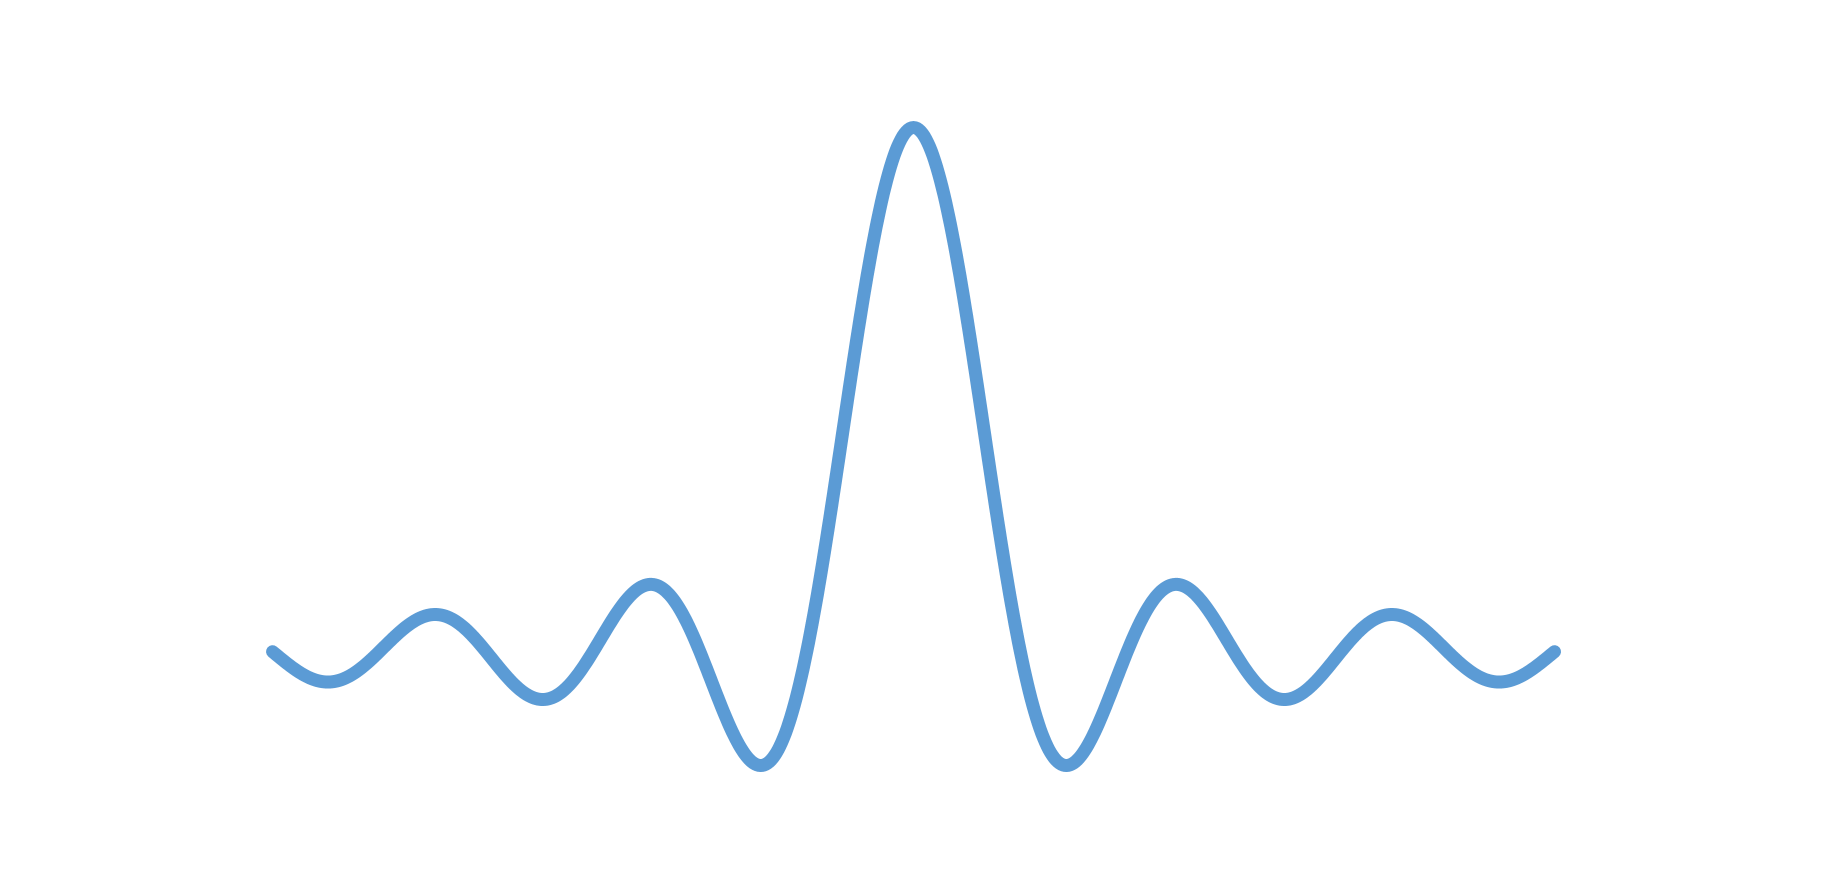
\includegraphics[width=4.00000cm]{./fig/sample.png} &
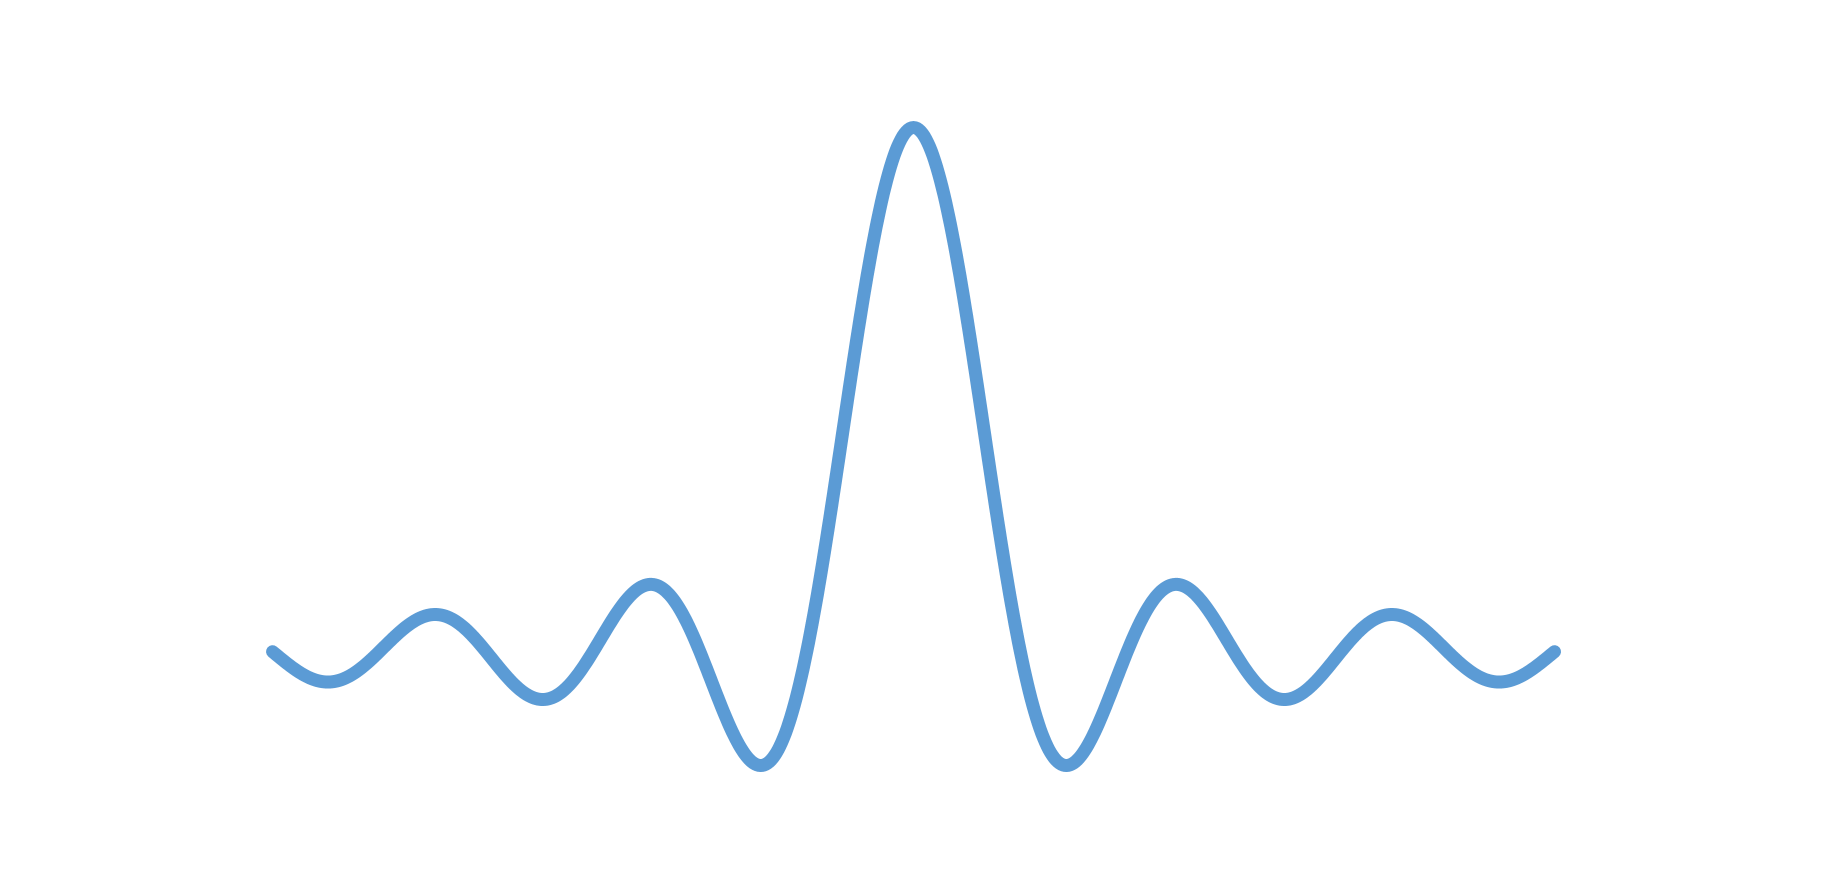
\includegraphics[width=4.00000cm]{./fig/sample.png}\\
(a) & (b)\\

\end{tabular}
\caption{test2}
\end{figure}

\section{数式}\label{ux6570ux5f0f}

スクリプトにてalign環境へ変換済み. 文中でも数式\(y=ax^2\)は使える.

\begin{align}
y=ax^2
\end{align}

\section{表}\label{ux8868}

表\ref{tab:test}にテスト結果を示す.

\begin{table}[ht]
\caption{テスト結果\label{tab:test}}
\centering
\begin{tabular}[]{@{}cc@{}}





\toprule
たかし & ひろし\\
\midrule

67 & 86\\
72 & 66\\
\bottomrule
\end{tabular}

\end{table}

